\documentclass{report}
\usepackage[showframe=false]{geometry}
\usepackage{titlesec}
\usepackage{amsmath}
\usepackage{graphicx}

\pagenumbering{gobble}

\geometry{tmargin=60pt,bmargin=90pt,lmargin=90pt,
rmargin=90pt}

\titleformat{\chapter}{\normalfont\huge}{\thechapter.}{20pt}{\huge}
\titlespacing*{\chapter} {0pt}{0pt}{10pt}

\begin{document}

\chapter{Section 1}

Derive the analytical solution of $w_0$ and $w_1$

\vspace{5mm}

dataset: n=1, ..., N Observations

$x_n ->$ one dimensional variable

$t_n ->$ label

linear model: $f(x_n; w_0, w_1) = w_0+w_1*x_n$

squared loss function: $L = \frac{1}{N} \sum_{N} (f(x_n) - t_n)^2$

mean value of $x_n = \overline{x}$

mean value of $t_n = \overline{t_n}$

Helpful Equation: $\sum{N} x_n = N\overline{x_n}$

Helpful Equation: $\sum{N} t_n = N\overline{t_n}$

$$L = \frac{1}{N} \sum_{N} (w_0+w_1 x_n - t_n)^2$$
\begin{equation} \label{eq1}
\begin{split}
\frac{\partial L}{\partial w_0} & = \frac{1}{N} \sum_{N} 2(w_0+w_1 x_n - t_n) \\
                                & = \frac{2}{N} \sum_{N} (w_0+w_1 x_n - t_n) = 0 \\
                                & = \frac{2}{N} (\sum_{N}w_0 + \sum_{N}w_1 x_n - \sum_{N}t_n) = 0 \\
                                & = \frac{2\sum_{N}w_0}{N} + \frac{2\sum_{N}w_1 x_n}{N} - \frac{2\sum_{N}t_n}{N} = 0 \\
                                & = \frac{2Nw_0}{N} + \frac{2w_1N\overline{x_n}}{N} - \frac{2N\overline{t_n}}{N} = 0 \\
                                & = 2w_0 + 2w_1\overline{x_n} - 2\overline{t_n} = 0
\end{split}
\end{equation}

\begin{equation} \label{eq2}
\begin{split}
\frac{\partial L}{\partial w_1} & = \frac{1}{N} \sum_{N} 2(w_0+w_1 x_n - t_n)x_n      \\
                                & = \frac{2}{N} \sum_{N} (w_0+w_1 x_n - t_n)x_n = 0 \\
                                & = \frac{2}{N} (\sum_{N}w_0 x_n + \sum_{N}w_1 x_n^2- \sum_{N}t_nx_n) = 0 \\
                                & = \frac{2}{N} (w_0\sum_{N} x_n + w_1\sum_{N} x_n^2- \sum_{N}t_nx_n) = 0 \\
                                & = \frac{2w_0\sum_{N}x_n}{N} + \frac{2w_1\sum_{N}x_n^2}{N}- \frac{2\sum_{N}t_nx_n}{N} = 0 \\
                                & = \frac{2w_0N\overline{x_n}}{N} + \frac{2w_1N\overline{x_n^2}}{N}- \frac{2N\overline{t_nx_n}}{N} = 0 \\
                                & = 2w_0\overline{x_n} + 2w_1\overline{x_n^2} - 2\overline{t_nx_n} = 0
\end{split}
\end{equation}

\begin{equation} \label{eq3}
\begin{split}
\frac{\partial L}{\partial w_0} & = 2w_0 + 2w_1\overline{x_n} - 2\overline{t_n} = 0 \\
\frac{\partial L}{\partial w_1} & = 2w_0\overline{x_n} + 2w_1\overline{x_n^2} - 2\overline{t_nx_n} = 0
\end{split}
\end{equation}

\begin{equation} \label{eq3}
\begin{split}
w_0 & = \frac{\overline{x_n}\overline{t_n} - \overline{x_nt_n}}{\overline{x_n}^2 - \overline{x_n^2}} \\
w_1 & = \overline{t_n} - \overline{x_n}\frac{\overline{x_n}\overline{t_n} - \overline{x_nt_n}}{\overline{x_n}^2 - \overline{x_n^2}}
\end{split}
\end{equation}

\chapter{Section 2}

Derive the analytical solution of $w$ in vector and matrix format

\vspace{5mm}

dataset: n=1, ..., N Observations

$W = [w_0, w_1]^T$

$X_n = [1, x_n]^T$

linear model: $f(x_n; w_0, w_1) = w_0+w_1*x_n = W^TX_n$

squared loss function: $L = \frac{1}{N} \sum_{N} (f(x_n) - t_n)^2$

$$L = \frac{1}{2N} \sum_{N} (W^TX_n - t_n)^2$$

\begin{equation} \label{eq1}
\begin{split}
L & = \frac{1}{N} \sum_{N} (W^TX_n - t_n)^2\\
  & = \frac{1}{N} (X_nW - t_n)^T(X_nW-t_n) \\
  & = ((X_nW)^T - t_n^T)(X_nW-t_n) \\
  & = (X_nW)^T X_nW - (X_nW)^Tt_n - t_n^T(X_nW) + t_n^Tt_n \\
  & = W^TX_n^TX_nW - 2(X_nW)^Tt_n + t_n^Tt_n
\end{split}
\end{equation}

\begin{equation} \label{eq2}
\begin{split}
\frac{\partial L}{\partial W}  & = 2X_n^TX_nW - 2X_n^Tt_n = 0 \\
                               & = X_n^TX_nW = X_n^Tt_n \\
                               & = (X_n^TX_n)^{-1}X_n^Tt_n
\end{split}
\end{equation}

\chapter{Section 3}
Discuss the selection of L2-norm vs L1-norm as the loss function for linear modeling (regression). You are asked to use examples of justify your answer.

When comparing L2 and L1 norms one of the biggest differences comes when your data contains some form of outliers. If your data does contain outliers then the L1 norm is going to move a much grater distance towards that outlier then the L2 norm would. A good example of this is shown in the figure below. As you can see when an outlier is introduced L1 is pulled more into the direction of the outlier then L2 is. In practice L2 is used much more then L1.

\begin{figure}[h!]
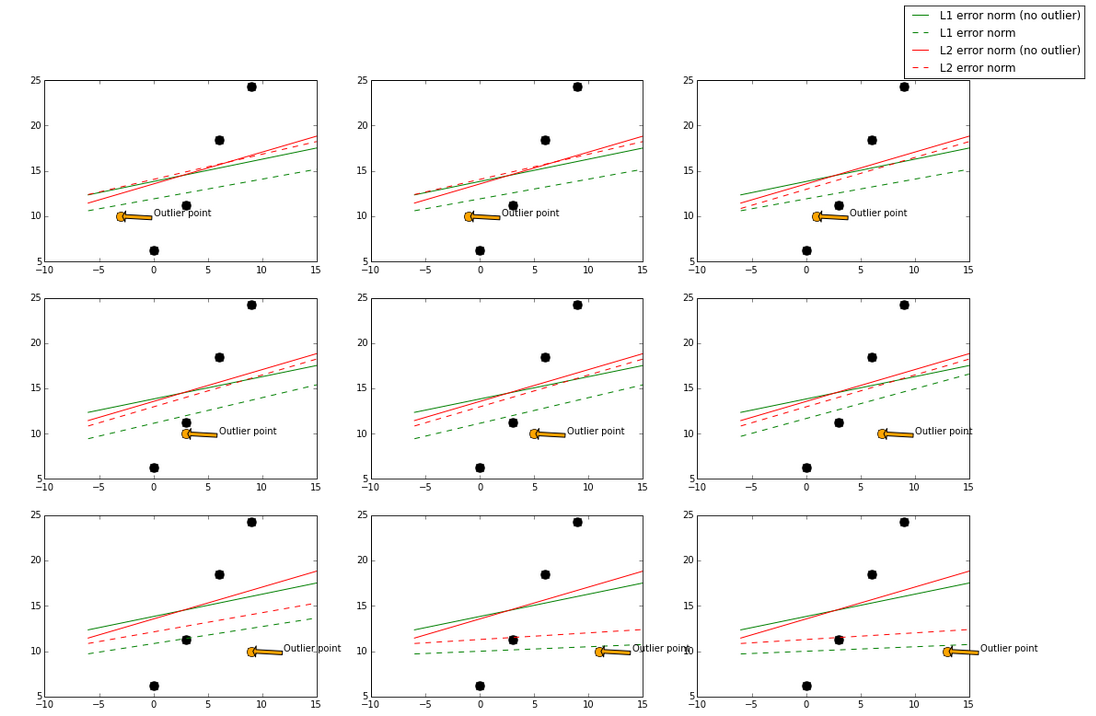
\includegraphics[width=\linewidth]{programmatic-L1-vs-L2-visualization.png}
\caption{programmatic-L1-vs-L2-visualization}
\label{fig:programmatic-L1-vs-L2-visualization}
\end{figure}

\chapter{Section 4}
S = {(1, 1), (2, 2), (3, 3)}

$$w_0 = 0$$
$$w_1 = 0$$
Step size = 0.1
$$f(x) = w_0+w_1*x_n$$

Gradient Descent Equation: $w_j - \alpha \frac{2}{N} \sum_{N }(w_0 + w_1*x_n-t_n)x_n$

Stochastic Gradient Descent Equation: $w_j - \alpha (w_0 + w_1*xₙ-t_n)x_n$

Gradient Descent
\begin{equation} \label{eq1}
\begin{split}
n & = 1\\
w_0 & = 0 - 0.1 * 2/3 * -6 = 0.4\\
w_1 & = 0 - 0.1 * 2/3 * -14 = 0.933333333333333\\
n & = 2\\
w_0 & = 0.4 - 0.1 * 2/3 * 0.8 = 0.346666666666667\\
w_1 & = 0.933333333333333 - 0.1 * 2/3 * 1.46666666666667 = 0.835555555555556\\
n & = 3\\
w_0 & = 0.346666666666667 - 0.1 * 2/3 * 0.0533333333333337 = 0.343111111111111\\
w_1 & = 0.835555555555556 - 0.1 * 2/3 * -0.222222222222221 = 0.85037037037037\\
n & = 4\\
w_0 & = 0.343111111111111 - 0.1 * 2/3 * 0.131555555555555 = 0.334340740740741\\
w_1 & = 0.85037037037037 - 0.1 * 2/3 * -0.0361481481481489 = 0.85278024691358\\
n & = 5\\
w_0 & = 0.334340740740741 - 0.1 * 2/3 * 0.119703703703703 = 0.32636049382716\\
w_1 & = 0.85278024691358 - 0.1 * 2/3 * -0.0550320987654327 = 0.856449053497942\\
n & = 6\\
w_0 & = 0.32636049382716 - 0.1 * 2/3 * 0.117775802469136 = 0.318508773662551\\
w_1 & = 0.856449053497942 - 0.1 * 2/3 * -0.0515502880658443 = 0.859885739368999\\
n & = 7\\
w_0 & = 0.318508773662551 - 0.1 * 2/3 * 0.114840757201646 = 0.310852723182442\\
w_1 & = 0.859885739368999 - 0.1 * 2/3 * -0.0505470068587099 = 0.863255539826246\\
n & = 8\\
w_0 & = 0.310852723182442 - 0.1 * 2/3 * 0.112091408504801 = 0.303379962615455\\
w_1 & = 0.863255539826246 - 0.1 * 2/3 * -0.0493061033379059 = 0.866542613382106\\
n & = 9\\
w_0 & = 0.303379962615455 - 0.1 * 2/3 * 0.109395568139004 = 0.296086924739521\\
w_1 & = 0.866542613382106 - 0.1 * 2/3 * -0.0481236369577798 = 0.869750855845958\\
\end{split}
\end{equation}
\begin{equation} \label{eq1}
\begin{split}
n & = 10\\
w_0 & = 0.296086924739521 - 0.1 * 2/3 * 0.106765909294315 = 0.288969197453234\\
w_1 & = 0.869750855845958 - 0.1 * 2/3 * -0.0469664697194532 = 0.872881953827255\\
n & = 11\\
w_0 & = 0.288969197453234 - 0.1 * 2/3 * 0.104199315323233 = 0.282022576431685\\
w_1 & = 0.872881953827255 - 0.1 * 2/3 * -0.045837461699024 = 0.87593778460719\\
n & = 12\\
w_0 & = 0.282022576431685 - 0.1 * 2/3 * 0.101694436938197 = 0.275242947302472\\
w_1 & = 0.87593778460719 - 0.1 * 2/3 * -0.0447355569092258 = 0.878920155067805\\
n & = 13\\
w_0 & = 0.275242947302472 - 0.1 * 2/3 * 0.0992497723142469 = 0.268626295814855\\
w_1 & = 0.878920155067805 - 0.1 * 2/3 * -0.0436601452358956 = 0.881830831416865\\
n & = 14\\
w_0 & = 0.268626295814855 - 0.1 * 2/3 * 0.0968638759457556 = 0.262168704085138\\
w_1 & = 0.881830831416865 - 0.1 * 2/3 * -0.0426105852747589 = 0.884671537101849\\
n & = 15\\
w_0 & = 0.262168704085138 - 0.1 * 2/3 * 0.0945353348665081 = 0.255866348427371\\
w_1 & = 0.884671537101849 - 0.1 * 2/3 * -0.041586256063286 = 0.887443954172735\\
n & = 16\\
w_0 & = 0.255866348427371 - 0.1 * 2/3 * 0.092262770318521 = 0.249715497072803\\
w_1 & = 0.887443954172735 - 0.1 * 2/3 * -0.0405865510174885 = 0.890149724240567\\
n & = 17\\
w_0 & = 0.249715497072803 - 0.1 * 2/3 * 0.0900448366618125 = 0.243712507962015\\
w_1 & = 0.890149724240567 - 0.1 * 2/3 * -0.0396108781952402 = 0.892790449453583\\
n & = 18\\
w_0 & = 0.243712507962015 - 0.1 * 2/3 * 0.087880220607546 = 0.237853826588179\\
w_1 & = 0.892790449453583 - 0.1 * 2/3 * -0.0386586598777414 = 0.895367693445433\\
n & = 19\\
w_0 & = 0.237853826588179 - 0.1 * 2/3 * 0.0857676404371335 = 0.23213598389237\\
w_1 & = 0.895367693445433 - 0.1 * 2/3 * -0.0377293322348675 = 0.897882982261091\\
n & = 20\\
w_0 & = 0.23213598389237 - 0.1 * 2/3 * 0.0837058452436541 = 0.22655559420946\\
w_1 & = 0.897882982261091 - 0.1 * 2/3 * -0.0368223449905105 = 0.900337805260458\\
\end{split}
\end{equation}

\begin{equation} \label{eq1}
\begin{split}
w_0 & ~ 2.2\\
w_1 & ~ 0.90\\
\end{split}
\end{equation}

Stochastic Gradient Descent
\begin{equation} \label{eq1}
\begin{split}
  n & = 1 \\
w_0 & = 0 - 0.1 * (0+0*1-1) * 1 = 0.1\\
w_1 & = 0 - 0.1 * (0+0*1-1) * 1 = 0.1\\
w_0 & = 0.1 - 0.1 * (0.1+0.1*2-2) * 1 = 0.27\\
w_1 & = 0.1 - 0.1 * (0.1+0.1*2-2) * 2 = 0.44\\
w_0 & = 0.27 - 0.1 * (0.27+0.44*3-3) * 1 = 0.411\\
w_1 & = 0.44 - 0.1 * (0.27+0.44*3-3) * 3 = 0.863\\
\end{split}
\end{equation}
\begin{equation} \label{eq1}
\begin{split}
  n & = 2 \\
w_0 & = 0.411 - 0.1 * (0.411+0.863*1-1) * 1 = 0.3836\\
w_1 & = 0.863 - 0.1 * (0.411+0.863*1-1) * 1 = 0.8356\\
w_0 & = 0.3836 - 0.1 * (0.3836+0.8356*2-2) * 1 = 0.37812\\
w_1 & = 0.8356 - 0.1 * (0.3836+0.8356*2-2) * 2 = 0.82464\\
w_0 & = 0.37812 - 0.1 * (0.37812+0.82464*3-3) * 1 = 0.392916\\
w_1 & = 0.82464 - 0.1 * (0.37812+0.82464*3-3) * 3 = 0.869028\\
\end{split}
\end{equation}
\begin{equation} \label{eq1}
\begin{split}
  n & = 3 \\
w_0 & = 0.392916 - 0.1 * (0.392916+0.869028*1-1) * 1 = 0.3667216\\
w_1 & = 0.869028 - 0.1 * (0.392916+0.869028*1-1) * 1 = 0.8428336\\
w_0 & = 0.3667216 - 0.1 * (0.3667216+0.8428336*2-2) * 1 = 0.36148272\\
w_1 & = 0.8428336 - 0.1 * (0.3667216+0.8428336*2-2) * 2 = 0.83235584\\
w_0 & = 0.36148272 - 0.1 * (0.36148272+0.83235584*3-3) * 1 = 0.375627696\\
w_1 & = 0.83235584 - 0.1 * (0.36148272+0.83235584*3-3) * 3 = 0.874790768\\
\end{split}
\end{equation}
\begin{equation} \label{eq1}
\begin{split}
n & = 4 \\
w_0 & = 0.375627696 - 0.1 * (0.375627696+0.874790768*1-1) * 1 = 0.3505858496\\
w_1 & = 0.874790768 - 0.1 * (0.375627696+0.874790768*1-1) * 1 = 0.8497489216\\
w_0 & = 0.3505858496 - 0.1 * (0.3505858496+0.8497489216*2-2) * 1 = 0.34557748032\\
w_1 & = 0.8497489216 - 0.1 * (0.3505858496+0.8497489216*2-2) * 2 = 0.83973218304\\
w_0 & = 0.34557748032 - 0.1 * (0.34557748032+0.83973218304*3-3) * 1 = 0.359100077376\\
w_1 & = 0.83973218304 - 0.1 * (0.34557748032+0.83973218304*3-3) * 3 = 0.880299974208\\
\end{split}
\end{equation}
\begin{equation} \label{eq1}
\begin{split}
  n & = 5 \\
w_0 & = 0.359100077376 - 0.1 * (0.359100077376+0.880299974208*1-1) * 1 = 0.3351600722176\\
w_1 & = 0.880299974208 - 0.1 * (0.359100077376+0.880299974208*1-1) * 1 = 0.8563599690496\\
w_0 & = 0.3351600722176 - 0.1 * (0.3351600722176+0.8563599690496*2-2) * 1 = 0.33037207118592\\
w_1 & = 0.8563599690496 - 0.1 * (0.3351600722176+0.8563599690496*2-2) * 2 = 0.84678396698624\\
w_0 & = 0.33037207118592 - 0.1 * (0.33037207118592+0.84678396698624*3-3) * 1 = 0.343299673971456\\
w_1 & = 0.84678396698624 - 0.1 * (0.33037207118592+0.84678396698624*3-3) * 3 = 0.885566775342848\\
\end{split}
\end{equation}
\begin{equation} \label{eq1}
\begin{split}
  n & = 6 \\
w_0 & = 0.343299673971456 - 0.1 * (0.343299673971456+0.885566775342848*1-1) * 1 = 0.320413029040026\\
w_1 & = 0.885566775342848 - 0.1 * (0.343299673971456+0.885566775342848*1-1) * 1 = 0.862680130411418\\
w_0 & = 0.320413029040026 - 0.1 * (0.320413029040026+0.862680130411418*2-2) * 1 = 0.31583570005374\\
w_1 & = 0.862680130411418 - 0.1 * (0.320413029040026+0.862680130411418*2-2) * 2 = 0.853525472438845\\
w_0 & = 0.31583570005374 - 0.1 * (0.31583570005374+0.853525472438845*3-3) * 1 = 0.328194488316712\\
w_1 & = 0.853525472438845 - 0.1 * (0.31583570005374+0.853525472438845*3-3) * 3 = 0.890601837227763\\
\end{split}
\end{equation}
\begin{equation} \label{eq1}
\begin{split}
n & = 7 \\
w_0 & = 0.328194488316712 - 0.1 * (0.328194488316712+0.890601837227763*1-1) * 1 = 0.306314855762264\\
w_1 & = 0.890601837227763 - 0.1 * (0.328194488316712+0.890601837227763*1-1) * 1 = 0.868722204673315\\
w_0 & = 0.306314855762264 - 0.1 * (0.306314855762264+0.868722204673315*2-2) * 1 = 0.301938929251375\\
w_1 & = 0.868722204673315 - 0.1 * (0.306314855762264+0.868722204673315*2-2) * 2 = 0.859970351651536\\
w_0 & = 0.301938929251375 - 0.1 * (0.301938929251375+0.859970351651536*3-3) * 1 = 0.313753930830777\\
w_1 & = 0.859970351651536 - 0.1 * (0.301938929251375+0.859970351651536*3-3) * 3 = 0.895415356389741\\
\end{split}
\end{equation}
\begin{equation} \label{eq1}
\begin{split}
n & = 8 \\
w_0 & = 0.313753930830777 - 0.1 * (0.313753930830777+0.895415356389741*1-1) * 1 = 0.292837002108725\\
w_1 & = 0.895415356389741 - 0.1 * (0.313753930830777+0.895415356389741*1-1) * 1 = 0.874498427667689\\
w_0 & = 0.292837002108725 - 0.1 * (0.292837002108725+0.874498427667689*2-2) * 1 = 0.288653616364314\\
w_1 & = 0.874498427667689 - 0.1 * (0.292837002108725+0.874498427667689*2-2) * 2 = 0.866131656178869\\
w_0 & = 0.288653616364314 - 0.1 * (0.288653616364314+0.866131656178869*3-3) * 1 = 0.299948757874222\\
w_1 & = 0.866131656178869 - 0.1 * (0.288653616364314+0.866131656178869*3-3) * 3 = 0.900017080708593\\
\end{split}
\end{equation}
\begin{equation} \label{eq1}
\begin{split}
n & = 9 \\
w_0 & = 0.299948757874222 - 0.1 * (0.299948757874222+0.900017080708593*1-1) * 1 = 0.279952174015941\\
w_1 & = 0.900017080708593 - 0.1 * (0.299948757874222+0.900017080708593*1-1) * 1 = 0.880020496850311\\
w_0 & = 0.279952174015941 - 0.1 * (0.279952174015941+0.880020496850311*2-2) * 1 = 0.275952857244285\\
w_1 & = 0.880020496850311 - 0.1 * (0.279952174015941+0.880020496850311*2-2) * 2 = 0.872021863306998\\
w_0 & = 0.275952857244285 - 0.1 * (0.275952857244285+0.872021863306998*3-3) * 1 = 0.286751012527757\\
w_1 & = 0.872021863306998 - 0.1 * (0.275952857244285+0.872021863306998*3-3) * 3 = 0.904416329157414\\
\end{split}
\end{equation}
\begin{equation} \label{eq1}
\begin{split}
n & = 10 \\
w_0 & = 0.286751012527757 - 0.1 * (0.286751012527757+0.904416329157414*1-1) * 1 = 0.26763427835924\\
w_1 & = 0.904416329157414 - 0.1 * (0.286751012527757+0.904416329157414*1-1) * 1 = 0.885299594988897\\
w_0 & = 0.26763427835924 - 0.1 * (0.26763427835924+0.885299594988897*2-2) * 1 = 0.263810931525536\\
w_1 & = 0.885299594988897 - 0.1 * (0.26763427835924+0.885299594988897*2-2) * 2 = 0.877652901321491\\
w_0 & = 0.263810931525536 - 0.1 * (0.263810931525536+0.877652901321491*3-3) * 1 = 0.274133967976535\\
w_1 & = 0.877652901321491 - 0.1 * (0.263810931525536+0.877652901321491*3-3) * 3 = 0.908622010674488\\
\end{split}
\end{equation}

\begin{equation} \label{eq1}
\begin{split}
w_0 & ~ 2.8\\
w_1 & ~ 0.90\\
\end{split}
\end{equation}



\end{document}
